\documentclass[12pt]{amsart}
\usepackage[margin=1in]{geometry}
\usepackage[english]{babel}
\usepackage[utf8]{inputenc}
\usepackage{subcaption}
\usepackage{amsmath}
\usepackage{amssymb}
\usepackage{amsfonts}
\usepackage{amsthm}
\usepackage{mathdots}
\usepackage{mathrsfs}
\usepackage[all]{xy}
\usepackage[pdftex]{graphicx}
\usepackage{color}
\usepackage{cite}
\usepackage{url}
\usepackage{indent first}
\usepackage[labelfont=bf,labelsep=period,justification=raggedright]{caption}
\usepackage[english]{babel}
\usepackage[utf8]{inputenc}
\usepackage{hyperref}
\usepackage[colorinlistoftodos]{todonotes}
\usepackage{tkz-fct}
\usepackage{tikz}
\usepackage{tikz-3dplot}
\usetikzlibrary{patterns}
\usetikzlibrary{calc}
\usetikzlibrary{knots}
\usetikzlibrary{spath3, intersections, hobby}
\usetikzlibrary{arrows, automata}
\usetikzlibrary{arrows.meta}
\usetikzlibrary{shapes.multipart}
\usetikzlibrary{topaths}
\usepackage{pgfplots}
\usepackage{multicol}
\PassOptionsToPackage{dvipsnames,svgnames}{xcolor}
\usepackage{textcomp}
\usepackage{bbm}
\usepackage{array}
\newcolumntype{C}{>{$}c<{$}}
\usepackage{forest}
\usepackage{tikzsymbols}
\usetikzlibrary{3d}
\tdplotsetmaincoords{80}{110}
\usepackage{worldflags}
\usepackage{youngtab}
\usepackage{tikzducks}

\makeatletter
\DeclareFontFamily{OMX}{MnSymbolE}{}
\DeclareSymbolFont{MnLargeSymbols}{OMX}{MnSymbolE}{m}{n}
\SetSymbolFont{MnLargeSymbols}{bold}{OMX}{MnSymbolE}{b}{n}
\DeclareFontShape{OMX}{MnSymbolE}{m}{n}{
    <-6>  MnSymbolE5
   <6-7>  MnSymbolE6
   <7-8>  MnSymbolE7
   <8-9>  MnSymbolE8
   <9-10> MnSymbolE9
  <10-12> MnSymbolE10
  <12->   MnSymbolE12
}{}
\DeclareFontShape{OMX}{MnSymbolE}{b}{n}{
    <-6>  MnSymbolE-Bold5
   <6-7>  MnSymbolE-Bold6
   <7-8>  MnSymbolE-Bold7
   <8-9>  MnSymbolE-Bold8
   <9-10> MnSymbolE-Bold9
  <10-12> MnSymbolE-Bold10
  <12->   MnSymbolE-Bold12
}{}

\let\llangle\@undefined
\let\rrangle\@undefined
\DeclareMathDelimiter{\llangle}{\mathopen}%
                     {MnLargeSymbols}{'164}{MnLargeSymbols}{'164}
\DeclareMathDelimiter{\rrangle}{\mathclose}%
                     {MnLargeSymbols}{'171}{MnLargeSymbols}{'171}
\makeatother

\makeatletter
\tikzoption{canvas is xy plane at z}[]{%
  \def\tikz@plane@origin{\pgfpointxyz{0}{0}{#1}}%
  \def\tikz@plane@x{\pgfpointxyz{1}{0}{#1}}%
  \def\tikz@plane@y{\pgfpointxyz{0}{1}{#1}}%
  \tikz@canvas@is@plane
}
\makeatother

\tikzset{surface/.style={draw=black, left color=orange,right color=orange,middle
color=orange!60!#1, fill opacity=1},surface/.default=white}

\newcommand{\coneback}[4][]{
  %% start at the correct point on the circle, draw the arc, then draw to the origin of the diagram, then close the path
  \draw[canvas is xy plane at z=#2, #1] (\tdplotmainphi-#4:#3) 
  arc(\tdplotmainphi-#4:\tdplotmainphi+180+#4:#3) -- (O) --cycle;
  }
\newcommand{\conefront}[4][]{
  \draw[canvas is xy plane at z=#2, #1] (\tdplotmainphi-#4:#3) arc
  (\tdplotmainphi-#4:\tdplotmainphi-180+#4:#3) -- (O) --cycle;
  }

\newcommand{\conetruncback}[6][]{
  \draw[line join=round,#1] plot[variable=\t,domain=\tdplotmainphi-#4:\tdplotmainphi+180+#4] 
  ({#3*cos(\t)},{#3*sin(\t)},#2)
  -- plot[variable=\t,domain=\tdplotmainphi+180-#4:\tdplotmainphi+#4] 
  ({#6*cos(\t)},{#6*sin(\t)},#5)
  --cycle;
  }

\newcommand{\conetruncfront}[6][]{
  \draw[line join=round,#1] plot[variable=\t,domain=\tdplotmainphi-#4:\tdplotmainphi-180+#4] 
  ({#3*cos(\t)},{#3*sin(\t)},#2)
  -- plot[variable=\t,domain=\tdplotmainphi-180-#4:\tdplotmainphi+#4] 
  ({#6*cos(\t)},{#6*sin(\t)},#5)
  --cycle;
  }

\pgfplotsset{compat=1.17}

% \topmargin 0.4cm
% \oddsidemargin 0.5cm
% \evensidemargin 0.5cm
% \textwidth 14cm 
% \textheight 20.2cm

% \setlength{\oddsidemargin}{0.25in}
% \setlength{\evensidemargin}{0.25in}
% \setlength{\textwidth}{6in}
%\setlength{\topmargin}{-0.25in}
%\setlength{\textheight}{8in}

\DeclareMathOperator{\ab}{ab}
\DeclareMathOperator{\sttt}{\text{st}}
\DeclareMathOperator{\Area}{Area}
\DeclareMathOperator{\atan}{atan}
\DeclareMathOperator{\Aut}{Aut}
\DeclareMathOperator{\BGL}{BGL}
\DeclareMathOperator{\Br}{Br}
\DeclareMathOperator{\card}{card}
\DeclareMathOperator{\ch}{ch}
\DeclareMathOperator{\Char}{char}
\DeclareMathOperator{\CHur}{CHur}
\DeclareMathOperator{\Cl}{Cl}
\DeclareMathOperator{\coker}{coker}
\DeclareMathOperator{\Conf}{Conf}
\DeclareMathOperator{\Cyc}{\textsc{Cyc}}
\DeclareMathOperator{\disc}{disc}
\DeclareMathOperator{\dist}{dist}
\DeclareMathOperator{\End}{End}
\DeclareMathOperator{\et}{\text{\'et}}
\DeclareMathOperator{\even}{even}
\DeclareMathOperator{\Fix}{Fix}
\DeclareMathOperator{\Gal}{Gal}
\DeclareMathOperator{\GL}{GL}
\DeclareMathOperator{\Hom}{Hom}
\DeclareMathOperator{\Hur}{Hur}
\DeclareMathOperator{\im}{im}
\DeclareMathOperator{\Ind}{Ind}
\DeclareMathOperator{\Inn}{Inn}
\DeclareMathOperator{\Int}{int}
\DeclareMathOperator{\Irr}{Irr}
\DeclareMathOperator{\lcm}{lcm}
\DeclareMathOperator{\mix}{mix}
\DeclareMathOperator{\Mor}{Mor}
\DeclareMathOperator{\MSet}{\textsc{MSet}}
\DeclareMathOperator{\odd}{odd}
\DeclareMathOperator{\ord}{ord}
\DeclareMathOperator{\Out}{Out}
\DeclareMathOperator{\Perm}{Perm}
\DeclareMathOperator{\PGL}{PGL}
\DeclareMathOperator{\Pin}{Pin}
\DeclareMathOperator{\PSet}{\textsc{PSet}}
\DeclareMathOperator{\PSL}{PSL}
\DeclareMathOperator{\rad}{rad}
\DeclareMathOperator{\rel}{rel}
\DeclareMathOperator{\Root}{root}
\DeclareMathOperator{\sech}{sech}
\DeclareMathOperator{\Seq}{\textsc{Seq}}
\DeclareMathOperator{\Set}{\textsc{Set}}
\DeclareMathOperator{\SL}{SL}
\DeclareMathOperator{\SO}{SO}
\DeclareMathOperator{\Spec}{Spec}
\DeclareMathOperator{\Spin}{Spin}
\DeclareMathOperator{\St}{St}
\DeclareMathOperator{\Surj}{Surj}
\DeclareMathOperator{\Syl}{Syl}
\DeclareMathOperator{\tame}{tame}
\DeclareMathOperator{\Tr}{Tr}
\DeclareMathOperator{\TV}{TV}
\DeclareMathOperator{\UCyc}{\textsc{UCyc}}
\DeclareMathOperator{\Var}{Var}

\newcommand{\eps}{\varepsilon}
\newcommand{\stt}{{}^*}
\newcommand{\QED}{\hspace{\stretch{1}} $\blacksquare$}
\renewcommand{\AA}{\mathbb{A}}
\newcommand{\BB}{\mathbb{B}}
\newcommand{\CC}{\mathbb{C}}
\newcommand{\EE}{\mathbb{E}}
\newcommand{\FF}{\mathbb{F}}
\newcommand{\HH}{\mathbb{H}}
\newcommand{\NN}{\mathbb{N}}
\newcommand{\OO}{\mathbb{O}}
\newcommand{\PP}{\mathbb{P}}
\newcommand{\QQ}{\mathbb{Q}}
\newcommand{\RR}{\mathbb{R}}
\renewcommand{\SS}{\mathbb{S}}
\newcommand{\ZZ}{\mathbb{Z}}
\newcommand{\bfa}{\mathbf{a}}
\newcommand{\bfb}{\mathbf{b}}
\newcommand{\bfc}{\mathbf{c}}
\newcommand{\bfd}{\mathbf{d}}
\newcommand{\bfe}{\mathbf{e}}
\newcommand{\bfm}{\mathbf{m}}
\newcommand{\bfn}{\mathbf{n}}
\newcommand{\bfN}{\mathbf{N}}
\newcommand{\bfp}{\mathbf{p}}
\newcommand{\bfq}{\mathbf{q}}
\newcommand{\bft}{\mathbf{t}}
\newcommand{\bfv}{\mathbf{v}}
\newcommand{\bfw}{\mathbf{w}}
\newcommand{\mcA}{\mathcal{A}}
\newcommand{\mcB}{\mathcal{B}}
\newcommand{\mcC}{\mathcal{C}}
\newcommand{\mcD}{\mathcal{D}}
\newcommand{\mcE}{\mathcal{E}}
\newcommand{\mcF}{\mathcal{F}}
\newcommand{\mcG}{\mathcal{G}}
\newcommand{\mcH}{\mathcal{H}}
\newcommand{\mcI}{\mathcal{I}}
\newcommand{\mcJ}{\mathcal{J}}
\newcommand{\mcK}{\mathcal{K}}
\newcommand{\mcL}{\mathcal{L}}
\newcommand{\mcM}{\mathcal{M}}
\newcommand{\mcN}{\mathcal{N}}
\newcommand{\mcO}{\mathcal{O}}
\newcommand{\mcP}{\mathcal{P}}
\newcommand{\mcQ}{\mathcal{Q}}
\newcommand{\mcR}{\mathcal{R}}
\newcommand{\mcS}{\mathcal{S}}
\newcommand{\mcT}{\mathcal{T}}
\newcommand{\mcU}{\mathcal{U}}
\newcommand{\mcW}{\mathcal{W}}
\newcommand{\mcX}{\mathcal{X}}
\newcommand{\mcY}{\mathcal{Y}}
\newcommand{\mcZ}{\mathcal{Z}}
\newcommand{\mfa}{\mathfrak{a}}
\newcommand{\mfb}{\mathfrak{b}}
\newcommand{\mfc}{\mathfrak{c}}
\newcommand{\mfI}{\mathfrak{I}}
\newcommand{\mfK}{\mathfrak{K}}
\newcommand{\mfM}{\mathfrak{M}}
\newcommand{\mfm}{\mathfrak{m}}
\newcommand{\mfo}{\mathfrak{o}}
\newcommand{\mfO}{\mathfrak{O}}
\newcommand{\mfP}{\mathfrak{P}}
\newcommand{\mfp}{\mathfrak{p}}
\newcommand{\mfq}{\mathfrak{q}}
\newcommand{\mfz}{\mathfrak{z}}
\newcommand{\msC}{\mathscr{C}}
\newcommand{\msP}{\mathscr{P}}
\newcommand{\AGL}{\mathbb{A}\GL}
\newcommand{\Qbar}{\overline{\QQ}}
\renewcommand{\qedsymbol}{$\blacksquare$}
\newcommand{\bbone}{\mathbbm{1}}

\newcommand{\bgamma}{\boldsymbol{\gamma}}
\newcommand{\bdelta}{\boldsymbol{\delta}}
\newcommand{\bpi}{\boldsymbol{\pi}}
\newcommand{\bsigma}{\boldsymbol{\sigma}}

\newcommand\TikCircle[1][2.5]{{\mathop{\tikz[baseline=-#1]{\draw[thick](0,0)circle[radius=#1mm];}}}}

\newcommand*\circled[1]{\tikz[baseline=(char.base)]{
            \node[shape=circle,draw,inner sep=2pt] (char) {#1};}}

\DeclareRobustCommand{\sstirling}{\genfrac\{\}{0pt}{}}
\DeclareRobustCommand{\fstirling}{\genfrac[]{0pt}{}}
\def\multiset#1#2{\ensuremath{\left(\kern-.3em\left(\genfrac{}{}{0pt}{}{#1}{#2}\right)\kern-.3em\right)}}
\DeclareRobustCommand{\eulerian}{\genfrac\langle\rangle{0pt}{}}

\newcommand{\planefig}[2] {
\filldraw[shift={#1},rotate=#2] (.4,.3) circle (2pt);
\filldraw[shift={#1},rotate=#2] (-.4,.3) circle (2pt);
\draw[shift={#1},rotate=#2] (-20:.55) arc (-20:-160:.55);
\draw[shift={#1},rotate=#2] (0,0) circle (1cm);
}

\makeatletter
\let\pgfnodeparttrbox\pgfnodeparttwobox
\let\pgfnodepartblbox\pgfnodepartthreebox
\let\pgfnodepartbrbox\pgfnodepartfourbox
\newif\ifpgfcirclecrosssplitcustomfill
\tikzset{%
  circle cross split part fill/.code=\def\pgf@lib@sh@ccs@list@fill{#1}\pgfcirclecrosssplitcustomfilltrue,%
  circle cross split uses custom fill/.is if=pgfcirclecrosssplitcustomfill}
\pgfdeclareshape{circle cross split}{%
  \nodeparts{text,two,three,four}%
  \savedanchor\centerpoint{%
    \pgfmathsetlength\pgf@xa{\pgfkeysvalueof{/pgf/inner xsep}}%
    \pgfmathsetlength\pgf@ya{\pgfkeysvalueof{/pgf/inner ysep}}%
    \pgf@x\wd\pgfnodeparttextbox
    \pgf@yb\dp\pgfnodeparttextbox
    \pgf@yc\dp\pgfnodeparttwobox
    \ifdim\pgf@yb>\pgf@yc
      \pgf@yc\pgf@yb
    \fi
    \advance\pgf@y-\pgf@yc
    \advance\pgf@x\pgf@xa
    \advance\pgf@y-\pgf@ya
    \advance\pgf@x.5\pgflinewidth
    \advance\pgf@y-.5\pgflinewidth
  }%
  \savedanchor\twoanchor{%
    \pgfmathsetlength\pgf@xa{\pgfkeysvalueof{/pgf/inner xsep}}%
    \pgfmathsetlength\pgf@ya{\pgfkeysvalueof{/pgf/inner ysep}}%
    \advance\pgf@x.5\pgflinewidth
    \advance\pgf@x\pgf@xa
    \advance\pgf@y.5\pgflinewidth
    \advance\pgf@y\pgf@ya
    \pgf@yb\dp\pgfnodeparttextbox
    \pgf@yc\dp\pgfnodeparttwobox
    \ifdim\pgf@yb>\pgf@yc
      \pgf@yc\pgf@yb
    \fi
    \advance\pgf@y\pgf@yc
  }%
  \savedanchor\threeanchor{%
    \pgfmathsetlength\pgf@ya{\pgfkeysvalueof{/pgf/inner ysep}}%
    \pgf@x\wd\pgfnodeparttextbox
    \pgf@yb\dp\pgfnodeparttextbox
    \pgf@yc\dp\pgfnodeparttwobox
    \ifdim\pgf@yb>\pgf@yc
      \pgf@yc\pgf@yb
    \fi
    \advance\pgf@y-\pgf@yc
    \advance\pgf@y-2\pgf@ya
    \advance\pgf@y-\pgflinewidth
    \pgf@yb\ht\pgfnodepartthreebox
    \pgf@yc\ht\pgfnodepartfourbox
    \ifdim\pgf@yb>\pgf@yc
      \pgf@yc\pgf@yb
    \fi
    \advance\pgf@y-\pgf@yc
    \advance\pgf@x-\wd\pgfnodepartthreebox
  }%
  \savedanchor\fouranchor{%
    \pgfmathsetlength\pgf@xa{\pgfkeysvalueof{/pgf/inner xsep}}%
    \advance\pgf@x\wd\pgfnodepartthreebox
    \advance\pgf@x2\pgf@xa
    \advance\pgf@x\pgflinewidth
  }%
  \saveddimen\radius{%
    % height:
    \pgf@y\ht\pgfnodeparttextbox
    \pgf@yb\ht\pgfnodeparttwobox
    \ifdim\pgf@yb>\pgf@y
      \pgf@y\pgf@yb
    \fi
    \pgf@yc\dp\pgfnodeparttextbox
    \pgf@yb\dp\pgfnodeparttwobox
    \ifdim\pgf@yc>\pgf@yb
      \advance\pgf@y\pgf@yc
    \else
      \advance\pgf@y\pgf@yb
    \fi
    \pgf@yb\ht\pgfnodepartthreebox
    \ifdim\pgf@yb<\ht\pgfnodepartfourbox
      \pgf@yb\ht\pgfnodepartfourbox
    \fi
    \pgf@yc\dp\pgfnodepartthreebox
    \ifdim\pgf@yc<\dp\pgfnodepartfourbox
      \advance\pgf@yb\dp\pgfnodepartfourbox
    \else
      \advance\pgf@yb\pgf@yc
    \fi
    \ifdim\pgf@yc>\pgf@y
      \pgf@y\pgf@yc
    \fi
    \pgfmathsetlength\pgf@ya{\pgfkeysvalueof{/pgf/inner ysep}}%
    \advance\pgf@y2\pgf@ya
    %
    \pgf@x\wd\pgfnodeparttextbox
    \pgf@xa\wd\pgfnodepartthreebox
    \pgf@xb\wd\pgfnodeparttwobox
    \pgf@xc\wd\pgfnodepartfourbox
    \ifdim\pgf@xa>\pgf@x
      \pgf@x\pgf@xa
    \fi
    \ifdim\pgf@xb>\pgf@x
      \pgf@x\pgf@xb
    \fi
    \ifdim\pgf@xc>\pgf@x
      \pgf@x\pgf@xc
    \fi
    \pgfmathsetlength\pgf@xa{\pgfkeysvalueof{/pgf/inner xsep}}%
    \advance\pgf@x2\pgf@xa
    \ifdim\pgf@y>\pgf@x
      \pgf@x\pgf@y
    \fi
    \advance\pgf@x.5\pgflinewidth
    %
    \pgfmathsetlength{\pgf@xb}{\pgfkeysvalueof{/pgf/minimum width}}%
    \pgfmathsetlength{\pgf@yb}{\pgfkeysvalueof{/pgf/minimum height}}%
    \ifdim\pgf@x<.5\pgf@xb
        \pgf@x=.5\pgf@xb
    \fi
    \ifdim\pgf@x<.5\pgf@yb
        \pgf@x=.5\pgf@yb
    \fi
    %
    \pgfmathsetlength{\pgf@xb}{\pgfkeysvalueof{/pgf/outer xsep}}%
    \pgfmathsetlength{\pgf@yb}{\pgfkeysvalueof{/pgf/outer ysep}}%
    \ifdim\pgf@xb<\pgf@yb
      \advance\pgf@x\pgf@yb
    \else
      \advance\pgf@x\pgf@xb
    \fi
  }%
  \inheritanchorborder[from=circle]%
  \inheritanchor[from=circle]{north}%
  \inheritanchor[from=circle]{north west}%
  \inheritanchor[from=circle]{north east}%
  \inheritanchor[from=circle]{center}%
  \inheritanchor[from=circle]{west}%
  \inheritanchor[from=circle]{east}%
  \inheritanchor[from=circle]{mid}%
  \inheritanchor[from=circle]{mid west}%
  \inheritanchor[from=circle]{mid east}%
  \inheritanchor[from=circle]{base}%
  \inheritanchor[from=circle]{base west}%
  \inheritanchor[from=circle]{base east}%
  \inheritanchor[from=circle]{south}%
  \inheritanchor[from=circle]{south west}%
  \inheritanchor[from=circle]{south east}%
  \anchor{two}{\twoanchor}%
  \anchor{three}{\threeanchor}%
  \anchor{four}{\fouranchor}%
  \inheritbackgroundpath[from=circle]
  \beforebackgroundpath{%
    \pgfutil@tempdima=\radius
    \pgfmathsetlength{\pgf@xb}{\pgfkeysvalueof{/pgf/outer xsep}}%  
    \pgfmathsetlength{\pgf@yb}{\pgfkeysvalueof{/pgf/outer ysep}}%  
    \ifdim\pgf@xb<\pgf@yb
      \advance\pgfutil@tempdima by-\pgf@yb
    \else
      \advance\pgfutil@tempdima by-\pgf@xb
    \fi
    \advance\pgfutil@tempdima by-.5\pgflinewidth%
    \pgfsetshortenstart{0pt}%
    \pgfsetshortenend{0pt}%
    \pgfsetarrows{-}%  
    \pgfpathmoveto{\pgfpointadd{\centerpoint}{\pgfqpoint{-\pgfutil@tempdima}{0pt}}}%
    \pgfpathlineto{\pgfpointadd{\centerpoint}{\pgfqpoint{\pgfutil@tempdima}{0pt}}}%
    \pgfpathmoveto{\pgfpointadd{\centerpoint}{\pgfqpoint{0pt}{-\pgfutil@tempdima}}}%
    \pgfpathlineto{\pgfpointadd{\centerpoint}{\pgfqpoint{0pt}{\pgfutil@tempdima}}}%
    \pgfusepathqstroke
  }%
  \behindbackgroundpath{%
    \pgfutil@tempdima=\radius
    \pgfmathsetlength{\pgf@xb}{\pgfkeysvalueof{/pgf/outer xsep}}%  
    \pgfmathsetlength{\pgf@yb}{\pgfkeysvalueof{/pgf/outer ysep}}%  
    \ifdim\pgf@xb<\pgf@yb
      \advance\pgfutil@tempdima by-\pgf@yb
    \else
      \advance\pgfutil@tempdima by-\pgf@xb
    \fi
    \advance\pgfutil@tempdima by-.5\pgflinewidth%
    \ifpgfcirclecrosssplitcustomfill%
      \pgf@lib@sh@rs@process@list{\pgf@lib@sh@ccs@list@fill}{4}%
      {%
        \pgfmathloop
           \ifnum\pgfmathcounter>4%
           \else%
             \pgf@lib@sh@getalpha\pgf@lib@sh@rs@number{\pgfmathcounter}%
              \edef\pgf@tempa{\csname pgf@lib@sh@rs@\pgf@lib@sh@rs@number @item\endcsname}%
              \ifx\pgf@tempa\pgf@lib@sh@rs@nonetext\else
                \pgfsetfillcolor{\pgf@tempa}%
                \pgf@lib@sh@ccs@angles{\pgfmathcounter}%
                \pgfpathmoveto{\centerpoint}%
                \pgfpathlineto{\pgfpointadd{\centerpoint}{\pgfqpointpolar{\pgf@lib@sh@ccs@angle}{\pgfutil@tempdima}}}%
                \pgfpatharc{\pgf@lib@sh@ccs@angle}{\pgf@lib@sh@ccs@angle@}{\pgfutil@tempdima}%
                \pgfpathclose
                \pgfusepathqfill
              \fi
        \repeatpgfmathloop
      }%
    \fi%
  }%
}
\def\pgf@lib@sh@ccs@angles#1{%
  \ifcase#1\or\def\pgf@lib@sh@ccs@angle{90}%
           \or\def\pgf@lib@sh@ccs@angle{0}%
           \or\def\pgf@lib@sh@ccs@angle{180}%
           \else\def\pgf@lib@sh@ccs@angle{270}%
  \fi
  \edef\pgf@lib@sh@ccs@angle@{\number\numexpr\pgf@lib@sh@ccs@angle+90\relax}%
}
\makeatother

\newcommand{\simon}[1]{\todo[color=green]{SR: #1}}
\newcommand{\nitya}[1]{\todo[color=blue!30]{NM: #1}}
\newcommand{\penghui}[1]{\todo[color=red!60]{HPH: #1}}
\newcommand{\michael}[1]{\todo[color=yellow]{MW: #1}}
\newcommand{\winnie}[1]{\todo[color=purple!60]{WL: #1}}
\newcommand{\peter}[1]{\todo[color=pink]{PR: #1}}
\newcommand{\jae}[1]{\todo[color=brown!60]{JL: #1}}
\newcommand{\silas}[1]{\todo[color=orange]{SJ: #1}}

\theoremstyle{plain}
\newtheorem{thm}{Theorem}
\newtheorem{lemma}[thm]{Lemma}
\newtheorem{cor}[thm]{Corollary}
\newtheorem{conj}[thm]{Conjecture}
\newtheorem{prop}[thm]{Proposition}
\newtheorem{heur}[thm]{Heuristic}
\newtheorem{qn}[thm]{Question}
\newtheorem{claim}[thm]{Claim}

\theoremstyle{definition}
\newtheorem{defn}[thm]{Definition}
\newtheorem{cond}[thm]{Conditions}
\newtheorem*{notn}{Notation}

\theoremstyle{remark}
\newtheorem{rem}[thm]{Remark}
\newtheorem*{ex}{Example}
\newtheorem*{nonex}{Nonexample}
\newtheorem*{exer}{Exercise}

\theoremstyle{theorem}
\newtheorem*{axiom}{Zorn's Lemma}

\numberwithin{equation}{section}
\numberwithin{thm}{section}

\begin{document}

\title{Nonstandard Methods and Applications in Ramsey Theory}
\author{Yudhister KUmar}
\date{\today}
\email{cyclicalreasoning2021@gmail.com}
\maketitle


\begin{abstract}
    This is an expository paper in which we define nonstandard models, the transfer principle, and the basic properties of filters to construct the hyperreals, hyperintegers, and hypernaturals and prove the relevant properties of said systems. Subsequently, we reformulate and prove the Infinite Ramsey's Theorem, Hindman's Theorem, and Rado's Theorem using nonstandard methods. 
\end{abstract}

\section{Introduction}
Since the dawn of calculus, philosophical debates have ensued as to whether or not so-called \textit{infinitesimal} numbers exist. While the progenitors of calculus, Issac Newton and Gottfried Leibniz, developed methods which had provably correct results using fluid notions of what an ``infinitesimal" number actually is, the philosophical argument came to a head in the $19^{\text{th}}$ century, upon which the concept of a \textit{limit} was formed. The limit undergirds the rigorous notion of calculus we have today, and modern analysis is built on limits and epsilon-delta procedures.

However, a mathematician named Abraham Robinson in the early 1960s wanted to reformulate the rigor behind calculus in the terms of rigorously defined infinitesimal and infinitely large numbers. This led to the development of what we call today as \textit{nonstandard analysis}, and built upon previous nonstandard models of arithmetic which created number systems such as the hyperreals, hyperintegers, and hypernaturals which preserved the fundamental properties of the reals, integers, and naturals while adding infinite and infinitesimals to the mix. 

Today, these so-called nonstandard methods have been discovered to have wide-ranging applications, and this paper focuses on their applications to a field of mathematics known as Ramsey Theory. Ramsey theory deals with, on a fundamental level, order in large structures. A typical question in Ramsey theory is as follows: ``How big must some structure be to \textit{guarantee} that a particular property holds?" Nominally considered a branch of combinatorics, the applications of using nonstandard methods to prove theorems in Ramsey theory are numerous, especially using the special properties of the hypernatural numbers.

This paper begins with an introduction to nonstandard models and their properties (specifically the \textit{transfer principle}.) We then construct the hyperreals $\stt \RR$ with an ultrapower, and define key properties of filters and ultrafilters along the way. After that, we define the hyperintegers, hypernaturals, and showcase some key properties of their number systems. Then, we prove the Infinite Ramsey's Theorem using nonstandard methods with the hyperintegers and hypernaturals, and the more advanced Hindman's Theorem as well (which regards finite sums). Finally, the paper ends with a reformulation of the partition regularity of Diophantine equations in nonstandard ways, and a proof of Rado's theorem.

\section{Nonstandard Models and the Transfer Principle}
\begin{thm}[Existence of Nonstandard Models]
\label{nonstandardmodels} For every mathematical object $X,$ there exists a corresponding \textbf{nonstandard extension} (or hyperextension) $^*X$ such that all elementary properties of $X$ are preserved in $^*X,$ such that $^*X$ is not isomorphic to $X.$
\end{thm}
Here, we define a 1``mathematical object" to be anything that can be formally defined, including numbers, sets, functions, spaces, and even theorems and proofs in some cases. Specifically, it behooves us to consider:
\begin{enumerate}
    \item Real numbers and $k$-tuples of real numbers for every $k \in \NN,$
    \item All sets $A, B \subseteq \RR^k$ of real tuples, and all functions $f: A \rightarrow B$ between them,
    \item All sets made of objects in (1) and (2). This includes the families of functions $\mathscr{F} \subseteq \text{Fun}(\RR^k, \RR^h).$
\end{enumerate}The proof of this statement is well beyond the scope of this paper, and is a direct result of the L\"{o}wenheim-Skolem Theorem in model theory. Further reading can be found here \cite[Chapter 4]{Go98}.

Likewise, a similarly rigorous treatment is required to firmly define what an \textit{elementary property} is, but we can think of it roughly as any property which operates on the \textit{elements} of a given object $X,$ and can be expressed with finitely many logical operators solely on those elements. A standard example of this would be the associativity and commutativity of the real numbers $\RR$ under addition and multiplication, or the associativity of function composition for all functions $f: A \rightarrow B,$ where $A$ and $B$ are some sets. 

\textit{Nonelementary properties} are properties which can \textit{only} be expressed using more complex structures. For example, statements or properties concerning functions or subsets of the real numbers are not elementary to the real numbers. 
\begin{prop}[Archimedean Property of the Real Numbers]
\label{archimedeanproperty}
For all positive $x \in \RR$ there exists $n \in \NN$ such that $nx > 1.$
\end{prop}
\begin{rem}
The Archimedean Property is not an elementary property of the real numbers. 
\end{rem}
Notice that the formulation in \ref{archimedeanproperty} relies on the natural numbers $\NN,$ such that it is implied that $\NN \subset \RR.$ As this relies on on a logical structure "more advanced" than that of simply elemental relations, then this property is not elementary. If we try to express the Archimedean property in this manner, we get the following:
\begin{cor}[Archimedean Property of the Real Numbers]
    For all positive $x \in \RR$ either $x>1$ or $2x>1$ or $3x>1$ or $\ldots$ or $nx>1$ or \ldots
\end{cor}
This is not finite, so it is not elementary. 

\begin{thm}[Transfer Property]
\label{transferproperty} Let $P(X_1, \ldots , X_n)$ be an elementary property of the mathematical objects $X_1, \ldots , X_n.$ Then $P(X_1, \ldots , X_n)$ is true if and only if $P({}^*X_1, \ldots , {}^*X_n)$ is true:
\[ P(A_1, \ldots , A_n) \Longleftrightarrow P({}^*A_1, \ldots , {}^*A_n).\]
\end{thm}
We define the \textit{star map} as a function which associates some mathematical object $X$ to its associated nonstandard extension $^*X,$ and we list some of its relevant properties below. Assume $A, A_1, \ldots, A_n, B$ are sets, and $\mathscr{F}$ is some family of sets. Then we have:
\begin{enumerate}
    \item $a=b \iff \stt a = \stt b,$
    \item $a \in A \iff \stt a \in \stt A,$
    \item $\stt \emptyset = \emptyset,$
    \item $A \subseteq B \iff \stt A \subseteq \stt B,$
    \item $\stt (A \cup B) = \stt A \cup \stt B,$
    \item $\stt (A \cap B) = \stt A \cap \stt B,$
    \item $\stt (A \backslash B) = \stt A \backslash \stt B,$ where $A \backslash B$ is the set of elements of $A$ not in $B,$
    \item $\stt (a_1, \ldots , a_k) = (\stt a_1, \ldots , \stt a_n)$ where $(a_1, \ldots, a_k)$ is a tuple,
    \item $\stt ( A_1 , \ldots , A_n) = (\stt A_1, \ldots , \stt A_n),$
    \item $ \stt \{(a,a) \, | \, a \in A\} = \{(\xi, \xi) \, | \, \xi \in \stt A \,.$
    \item $\stt \{(x,y) \, | x \in y \in \mathscr{F} \} = \{(\xi,\zeta) \, | \xi \in \zeta \in \stt \mathscr{F} \},$
    \item $\stt\left(\bigcup _{F \in \mathscr F} F \right) = \bigcup _{G \in \stt \mathscr{F}}G.$
    
\end{enumerate}
\section{Filters}


\begin{defn}
A \textit{filter} over some nonempty set $I$ is a nonempty collection $\mathcal{F} \subseteq \mathcal{P}(I)$ such that:
\begin{itemize}
    \item if $A,B \in \mathcal{F},$ then $A \cap B \in \mathcal{F};$
    \item if $A \in \mathcal{F}$ and $A \subseteq B \subseteq I,$ then $B \in \mathcal{F}.$
\end{itemize}
Equivalently, $A \cap B \in \mathcal{F}$ if and only if $A,B \in \mcF.$
\end{defn}
A \textit{proper filter} is a filter $\mathcal{F}$ which does not contain the empty set $\emptyset.$ An \textit{ultrafilter} is a proper filter $\mathcal{U}$ such that for any $A \subseteq I,$ either $A$ or its complement $A^c$ (which is defined as $I \backslash A$) is a member of $\mathcal{U}.$ A \textit{principal ultrafilter} is an ultrafilter which contains a finite set, and a \textit{nonprincipal ultrafilter} only contains cofinite sets (a set is cofinite if its complement is finite).

\begin{defn}
The \textit{filter generated by $\mathcal{H}$} (denoted $\mathcal{F}^\mathcal{H}$) for some $\mathcal{H} \subseteq \mathcal{P}(I)$ is the collection
\[\mcF^\mcH = \{A \subseteq I: A\subseteq B_1 \cap \cdots \cap B_n \text{ for some $n \in \NN$ and some $B_i \in \mcH, \, 1 \leq i \leq n$}\}. \]
\end{defn}
When $\mcH$ has a single member $B,$ we call $\mcF^\mcH$ the \textit{principal filter generated by B}. When $B = \{i\}, i \in I$ \textemdash that is, $B$ has a single element\textemdash $\mcF^\mcH$ is the \textit{principal ultrafilter generated by i,} denoted by $\mcF^i.$
\begin{rem}
An ultrafilter is principal (contains a finite set) if and only if it contains a single element set. \label{seg}
\end{rem}
\begin{proof}
It is trivial in the forward direction. For the opposite, let $A \in \mcU,$ where $\mcU$ is some ultrafilter and $A$ is a finite set. For some element $a\in A,$ either $\{i\} \in \mcU$ or $\{i\}^c \in \mcU,$ by the definition of the ultrafilter. The former proves the claim, while the latter implies $A-i \in \mcU,$ where $A-i$ is the set of all elements of $A$ not including $i.$ By repeating the same process on $A-i,$ we recursively prove that the existence of a finite set in $\mcU$ implies the existence of a single element set, as one can continue this process until $A$ has two elements, and either $i$ or $A-i$ is a member of $\mcU$.
\end{proof}

\begin{defn}
A collection $\mathcal{H} \subseteq \mathcal{P}(I)$ has the \textit{finite intersection property} (abbreviated as FIP) if the intersection of every nonempty finite subcollection of $\mathcal{H}$ is nonempty. That is,
\[B_1 \cap \cdots \cap B_n \neq \emptyset \]
for all $n \in \mathbb{N}$ and all $B_1, \ldots, B_n \in \mathcal{H}.$ \label{fip}
\end{defn}
While this treatment of filters is enough for us to begin our construction of the hyperreals, we also need to state the axiom of choice in the form of Zorn's lemma.
\begin{axiom}
\label{zorn}
If $(P, \leq)$ is a partially ordered set in which every linearly ordered subset (or "chain") has an upper bound in $P,$ then $P$ contains a $\leq-$maximal element.
\end{axiom}
While specific discussion of the axiom of choice and its equivalents (namely: Zorn's lemma) is beyond the scope of this paper, this enables us to use the property of set inclusion $\subseteq$ as a partial ordering property. Any partial ordering property (denoted by $\leq$) must satisfy:
\begin{enumerate}
    \item Reflexivity: For some $a, a\leq a.$
    \item Antisymmetry: If $a \leq b$ and $b \leq a$ then $a = b.$
    \item Transitivity: If $a \leq b$ and $b \leq c$ then $a \leq c.$
\end{enumerate}
As the subset $\subseteq$ relation satisfies all three properties, it can be considered a partial ordering. 

\begin{thm}
Any collection of subsets of $I$ that has the finite intersection property can be extended to an ultrafilter on $I.$
\end{thm}
\begin{proof}
Let $\mcH$ be a collection of subsets of $I$ that has the FIP. Then, the filter $\mcF^\mcH$ is proper. Let $P$ be the collection of all proper filters on $I$ that include $\mcF^\mcH,$ partially ordered by set inclusion $\subseteq.$ Then, every linearly ordered subset of $P$ has an upper bound in $P,$ so \ref{zorn} implies $P$ has a maximal element, which is a maximal filter on $I$ and therefore an ultrafilter. 
\end{proof}
\begin{cor}
Any infinite set has a nonprincipal ultrafilter on it.
\end{cor}
\begin{proof}
If $I$ is infinite, the cofinite filter $\mcF^{co}$ is proper and has the finite intersection property, and so is included in an ultrafilter $\mcF.$ But for any $i \in I$ we have $I \backslash \{i\} \in \mcF^{co} \subseteq \mcF,$ so $\{i\} \not\in \mcF,$ whereas $\{i\} \in \mcF^{i}.$ Hence $\mcF \neq \mcF^i.$ Therefore, $\mcF$ is nonprincipal, as it is not equal to any principal ultrafilter. By \ref{seg}, all principal ultrafilters are of the form $\mcF^i.$
\end{proof}
This is the key insight we need to begin our construction of the hyperreals.
\section{Hyperreals}
\subsection{Introduction} The \textit{hyperreal} numbers $\stt \RR$ are a nonstandard extension of the real numbers, and they are useful because with them we are able to rigorously define what it means for a number to be an \textit{infinitesimal} or \textit{infinitely large.} That is, there exists some $\eps \in \stt \RR$ such that \[|\eps| < \frac{1}{n}\] for all $n \in \RR,$ and there exists some $\Omega \in \stt \RR$ such that \[| \Omega | > n\] for all $n \in \RR.$
\subsection{Construction of the Hyperreals}
Let $\RR^\NN$ be the set of all sequences of real numbers. A member $r \in \RR^\NN$ has the form $r = \langle r_n : n\in \NN \rangle,$ and we denote this by $r = \langle r_n \rangle.$ Addition and multiplication in $\RR^\NN$ are defined as follows, for $r,s \in \RR^\NN$: 
\begin{align*}
    r \oplus s &= \langle r_n + s_n : n\in \NN \rangle. \\
    r \otimes s &= \langle r_n \cdot s_n : n\in \NN \rangle.
\end{align*}
\begin{defn}
Let $r,s \in \RR^\NN$ be equivalent by the relation $\equiv$ such that
\[\langle r_n \rangle \equiv \langle s_n \rangle \text{ if and only if } \{n \in \NN : r_n = s_n \} \in \mcU\]
where $\mcU$ is some nonprincipal ultrafilter on $\NN.$ We call this relation \textit{almost everywhere agreement}, and it can be said that these two sequences agree on a ``large" set. Note that this holds when the agreement holds on some cofinite number of indices, as any cofinite set is in a nonprincipal ultrafilter.
\end{defn}
\begin{rem}
Note that $\equiv$ is an equivalence relation on $\RR^\NN.$
\end{rem}
Any equivalence relation (denoted by $\sim$) on $X$ satisfies three properties for $a,b,c \in X$:
\begin{itemize}
    \item Reflexivity: $a\sim a,$
    \item Symmetry: $a\sim b \iff b \sim a$
    \item Transitivity: If $a \sim b$ and $b \sim c $ then $a \sim c.$
\end{itemize}
From these, it is easy to see that $\equiv$ is an equivalence relation on $\RR^\NN.$

Typically, we set the agreement set $\{ n \in \NN : r_n = s_n\}$ as  $[[r = s]],$ and the equivalence class of some $r \in \RR^\NN$ will be denoted by $[r].$ From this, we can generate the quotient set of $\RR^\NN$ by $\equiv$ as 
\[^*\RR = \{[r] : r\in \RR^\NN\}.\]
Define, for $r,s \in \RR^\NN,$
\begin{align*}
    [r] +[s] &= [r \oplus s], \\
    [r]\cdot [s] &= [r\otimes s], \\
    [r] < [s] \iff [[r<s]] \in \mcU &\iff \{n\in \NN : r_n < s_n \} \in \mcU.
\end{align*}
These generalize the operations of addition and multiplication and ordering on $\RR^\NN$ to the hyperreals $\stt \RR$ by considering them in the context of equivalence classes and ''almost everywhere agreement." The sum and product of addition and multiplication respectively in the hyperreals give an equivalence class of $\RR^\NN,$, and we order elements of the hyperreals much like we establish their equivalence: if $r_n < s_n$ for almost all $n \in \NN,$ then $r < s,$ and we denote the agreement set of such as $[[r<s]].$ We now show that the hyperreals form a well ordered field.
\subsection{Properties of the Hyperreals}
\begin{defn}
\label{field}
A field is a set $\FF$ with two binary operations, normally called \textit{addition} and \textit{multiplication} and denoted respectively with $+$ and $\cdot,$ such that the following items hold for $a,b,c \in \FF$:
\begin{itemize}
    \item Associativity: $a + (b+c) = (a+b) + c,$ and $a \cdot (b \cdot c) = (a \cdot b) \cdot c,$
    \item Commutativity: $a + b = b + a,$ and $a \cdot b = b \cdot a,$
    \item Identities: There exist elements $0$ and $1$ in $\FF$ such that $a + 0 = a$ and $a \cdot 1 = a,$
    \item Additive Inverses: There exists a unique element $-a$ for every $a$ such that $a + (-a) = 0.$
    \item Multiplicative Inverses: There exists, for $a \neq 0,$ a unique element $a^{-1}$ such that $a \cdot a^{-1} = 1.$
    \item Distribution: $a \cdot (b+c) = (a\cdot b) + (a \cdot c).$
\end{itemize}
\end{defn}
\begin{thm}
$\stt \RR$ is a well-ordered field. \label{hyperrealfield}
\end{thm}
\begin{proof}
Associativity, commutativity, and distribution follow from the definitions of addition and multiplication in $\stt \RR.$ We define the additive identity $0 = \langle 0, 0, \ldots \rangle$ and the multiplicative identity $1 = \langle 1, 1, \ldots \rangle,$ which satisfy the necessary properties in $\stt \RR.$ Inverses can be constructed element-wise, such that for some $r=\langle r_1, r_2, \ldots \rangle$ you set $-r = \langle -r_1, -r_2, \ldots \rangle$ and similarly for multiplication. And as $\stt \RR$ has an ordering relation, it is a well-ordered field. 
\end{proof}
We now look at some interesting consequences of these properties. For instance, take 
\[a = \langle 1,2,3,\ldots \rangle, \]
\[b = \langle 2,2,3,\ldots \rangle.\]
We can say that $a$ and $b$ are equivalent in the hyperreals, as they agree at a \textit{large} number of instances (the agreement set is cofinite). However, the sequences 
\[c = \langle 1, \frac{1}{2}, \frac{1}{3}, \ldots \rangle\]
\[d = \langle 0, 0, 0, \ldots \rangle\]
are \textit{not} equivalent. Even though they are both approximated to $0$ (as we will be determined later), because their agreement set $[[c = d]]$ is \textit{empty} they are not equivalent. 
\begin{defn}
For every real number $c \in \RR,$ there exists a corresponding hyperreal number \[\stt c = \langle c, c, c, \ldots \rangle\]
such that for $a,b \in \RR$
\begin{itemize}
    \item $\stt (a+b) = \stt a + \stt b,$
    \item $\stt (a \cdot b) = \stt a \cdot \stt b,$
    \item $\stt a < \stt b \iff a < b,$
    \item $\stt a = \stt b \iff a = b.$
\end{itemize}
\end{defn}
\begin{thm}
There exists an infinitesimal $[\eps] \in \stt \RR$ such that $0 < \eps < r,$ for all $r \in \RR.$ \label{infinitesimal}
\end{thm}
\begin{proof}
Let $\eps = \langle 1, \frac{1}{2}, \frac{1}{3}, \ldots \rangle = \langle \frac{1}{n} \, | \, n \in \NN \rangle.$ Then, \[ [[ 0 < \eps ]] = \{n \in \NN \, | \, 0 < \frac{1}{n} \} = \NN \in \mcU,\] where $\mcU$ is a nonprincipal ultrafilter on $\NN.$ Therefore, $0 < [\eps].$ However, for any positve real number $r,$ the set 
\[[[\eps < r]] = \{n \in \NN \, | \, \frac{1}{n} < r \} \] is cofinite, and therefore $[[\eps < r]] \in \mcU$ because $\mcU$ is nonprincipal. Therefore, $[\eps]$ is an infinitesimal number.
\end{proof}

\begin{thm}
There exists an infinitely large hyperreal $[\Omega]$ such that for all $r \in \RR, [\Omega] > [r].$ \label{hyperreal}
\end{thm}
\begin{proof}
Set $\Omega = \langle 1,2,3,\ldots \rangle .$ Then, the agreement set 
\[[[\Omega > r]] = \{n \in \NN \, | \, n > r \}\] is cofinite and therefore in some nonprincipal ultrafilter $\mcU$ over $\NN.$ Therefore, it is a true statement, and $[\Omega]$ is an infinitely large hyperreal.
\end{proof}
Arguments like the ones in \ref{infinitesimal} and \ref{hyperreal} can be used to construct infinitely many infinitesimal and infinitely large numbers, but as the hyperreals are closed under addition this gives rise to the existence of infinitely many hyperreals between any two real numbers (as the result of adding infinitesimals and hyperreals). From this, our next result follows.
\begin{thm}[Standard Part]
Every finite number  $\xi \in \stt \RR$ has an infinitesimal difference from a unique real number. We denote this as the standard part of $\xi:$
\[\xi \approx \textnormal{st}(\xi) \in \RR. \]
\end{thm}
\begin{proof}
Let $A = \{r \in \RR \, | \, r < \xi \}.$ Since $\xi$ is finite, there exist real $r,s$ such that $r < \xi < s,$ so $A$ is nonempty and has a least upper bound $c \in \RR.$ We wish to show that $\xi$ is infinitely close to $c.$

Take any positive real $\eps \in \RR.$ If $c$ is the upper bound of $A,$ then $c + \eps\not\in A,$ so $\xi \leq c+\eps.$ If $\xi \leq c-\eps,$ then $c-\eps$ would be an upper bound of $A,$ so $c-\eps < \xi \leq c+\eps,$ which implies that $|\xi-c| \leq \eps.$ As $\eps$ is arbitrary, this holds for all positive real $\eps,$ so $\xi$ is infinitely close to $c.$ This proves the existence of $\text{st}(\xi) = c.$

For uniqueness, we consider a separate upper bound $c'.$ If $\xi \sim c$ and $c = c',$ then $\xi \sim c'.$ Therefore $\text{st}(\xi) = c$ is unique.
\end{proof}
From these, we see that the constructed hyperreals have the necessary properties to be a nonstandard extension of the real numbers (by \ref{hyperrealfield}) and contain infinitesimal and infinitely large numbers.

\section{Hyperintegers, Hypernaturals, and Iterated Hyper-Extensions}
\subsection{Construction of the Hyperintegers and Hypernaturals}
The floor function (also called integer part function) $\lfloor x \rfloor$ for $x \in \RR$ can be defined as $\max \{m \in \ZZ \, | \, m \leq x \}.$ There exists a nonstandard extension of the floor function $\stt \lfloor \cdot \rfloor$ which we can use to define the hyperintegers.
\begin{defn}
The hyperintegers $\stt \ZZ$ are the set of hyperreals such that they are equal to their own integer part, that is
\[\stt \ZZ = \{x \in \stt \RR \, | \, x = \stt \lfloor x \rfloor \}. \]
\end{defn}
From this, we can define the hypernaturals.
\begin{defn}
The hypernaturals $\stt \NN$ consist of all positive hyperintegers $\stt \ZZ.$
\end{defn}
These two number systems are the most useful when we consider applying nonstandard methods to more discrete areas of mathematics, and they have some interesting properties.

\subsection{Hyperfinite Sets}
For instance, take finite sets. We define a set $A$ to be finite if \[\#A \in \NN,\] where $\#A$ represents the cardinality of the set. Via the transfer principle, we can define \textit{hyperfinite} sets $\stt A$ such that \[\# \stt A \in \stt \NN.\]
\begin{prop}
For every $N, M \in \stt \NN$ such that $N < M,$
\[[N, M] _{\stt \NN} = \{v \in \stt \NN \, | \, N \leq v \leq M \} \] is a hyperfinite set.
\end{prop}
\subsection{Piecewise Syndetic Sets}
As an example of a concept which can be reformulated in a nonstandard manner, we take piecewise syndetic sets, which are normally defined as follows.
\begin{defn}
A set $A \subseteq \ZZ$ is \textit{thick} if for every $k \in \ZZ$ the interval $[x+1, x+k] \subseteq A.$
\end{defn}
\begin{defn}
A set $A \subseteq \ZZ$ is \textit{syndetic} if there exists $k \in \NN$ such that the interval $[x,x+k] \cap A \neq \emptyset$ for every $x \in \ZZ.$
\end{defn}
\begin{defn}
A set $A$ is \textit{piecewise syndetic} (denoted by PS) if $A = B \, \cap  \,C$ with $B$ syndetic and $C$ thick.
\end{defn}
However, we can define thick and syndetic sets with hyperextensions as well.
\begin{defn}
A set $A \in \ZZ$ is thick if $I \subset \stt A$ for some infinite interval $I.$
\end{defn}
\begin{defn}
A set $A$ is syndetic if $\stt A$ has finite gaps, formalized as \[\stt A \cup I \neq \emptyset\] for every infinite interval $I.$
\end{defn}
\begin{defn}
A set $A$ is piecewise syndetic if there exists an infinite interval $I$ such that $\stt A \cap I$ has finite gaps.
\end{defn}
\begin{prop}
Piecewise syndetic sets are partition regular: if a piecewise syndetic set is partitioned into finitely many pieces, then at least one of the pieces is piecewise syndetic.
\end{prop}
\begin{proof}
Let $A$ be some PS set, and let it be partitioned into two colorings $C_1, C_2$ such that $C_1 \, \cap \, C_2 = \emptyset$ and $A = C_1 \, \cup \, C_2.$ We take the hyperextension of this statement, so $\stt A =\stt C_1 \, \cup \, \stt C_2,$ and we pick an infinite interval $I$ where $\stt A$ has only finite gaps (exists by definition of PS). If $\stt C_1$ only has finite gaps in $I,$ then $C_1$ is PS. Otherwise, take the infinite interval $J \subseteq I$ such that $J \, \cap \, C_1 = \emptyset.$ Therefore, $J$ only contains elements of $C_2.$ However, $J$ has finite gaps, which means that $C_2$ only has finite gaps in $J.$ Therefore, $C_2$ is PS.
This argument for 2-colorings can be extended to $n$-colorings: for any colorings $C_1, \ldots , C_n$ take $C_1$ and $C_2, \ldots , C_n$ as a 2-coloring. Then, it follows that either is PS. If $C_1$ is not PS, repeat the same process with $C_2$ and so on.
\end{proof}
\subsection{Iterated Hyperextensions}
By the transfer principle, it is natural to consider the ``hyper-hypernaturals," or $\stt \stt \NN.$ These hyperextensions of hyperextensions exist, and they can be iterated successively, but to get a better understanding of their properties it is necessary to consider the hypernaturals as ultrafilters on $\NN.$
\begin{prop}
Every hypernatural number $\xi \in \stt N$ generates an ultrafilter on $\NN$ such that
\[\mcU_\xi = \{A \subseteq \NN \, | \, \xi \in \stt A \}. \]
\end{prop}
\begin{proof}
An ultrafilter must either contain a set or contain its complement. Let $A \subseteq \NN,$ and let $\mcU_\xi$ be the ultrafilter generated by $\xi.$ If $\xi \in \stt A,$ then $A \in \mcU_\xi.$ If $\xi \not\in \stt A,$ then $\xi \in \stt \NN \, \backslash \, \stt A,$ which by transfer has a counterpart $\NN \backslash A.$ As $\xi \in \stt ( \NN \backslash A), \, \mcU_\xi$ is an ultrafilter over $\NN,$ because for arbitrary $\xi, A$ it contains either $A$ or its complement $\NN \, \backslash \, A.$
\end{proof}
From this, we can establish a different notion of equivalence between hypernaturals: if the ultrafilter they generate is the same, then the hypernaturals can be considered the same.
\begin{defn}
For $\xi, \zeta \in \stt \NN,$ we say that $\xi$ and $\zeta$ are ``$u$-equivalent" (denoted by $\xi \underset{u}{\sim} \zeta)$ if they generate the same ultrafilter \[\mcU_\xi = \mcU_\zeta.\] 
\end{defn}
For every $A \subseteq \NN,$ either $\xi, \zeta \in \stt A$ or $\xi, \zeta \not \in \stt A$ (which follows from the definition of an ultrafilter).
\begin{defn}
Let $A$ be some set, and let $B$ be some subset of $A.$ $B$ is an \textit{initial segment} of $A$ if for some $x \in A, \, y \in B$ the statement $x < y$ implies that $x \in B.$
\end{defn}
\begin{prop}
The natural numbers are an initial segment of the hypernatural numbers, denoted by: \[ \NN < \stt \NN.\]
\end{prop}
\begin{proof}
For some natural number $n \in \NN,$ if for some $\Omega \in \stt \NN$ we have $\Omega < n,$ then $\Omega$ is finite and is a natural number. Therefore, $\NN$ is an initial segment of $\stt \NN.$
\end{proof}
\begin{cor}
The hypernatural numbers are an initial segment of the hyper-hypernaturals:
\[ \stt \NN < \stt \stt \NN. \]
\end{cor}
\begin{prop}
If $\xi \in \stt \NN \, \backslash \, \NN$ then $\stt \xi > \mu$ for all $\mu \in \stt N.$
\end{prop}
\begin{proof}
By transfer, $\stt \xi \in \stt \stt \NN \backslash \stt \NN,$ and as $\stt \NN$ is an initial segment of $\stt \NN,$ the proposition follows.
\end{proof}
\begin{defn}
If $\xi \in \stt \stt \NN,$ we define the ultrafilter generated by $\xi$ as \[\mcU_\xi = \{A \subseteq \NN \, | \, \xi \in \stt \stt A \}.\]
\end{defn}
\begin{thm}
For all $\xi \in \stt \NN, \stt \xi \underset{u}{\sim} \xi,$ so 
\[\mcU_{\stt \xi} = \mcU_\xi.\]
\end{thm}
\begin{proof}
We show that if and only if $A \in \mcU_\xi,$ then $\stt \xi \in \stt \stt A.$ In the foward direction, $A \in \mcU_\xi$ implies $\xi \in \stt A,$ which by transfer defines the truth of $\stt \xi \in \stt \stt A.$ In the reverse direction, $\stt \xi \in \stt \stt A$ by transfer implies $\xi \in \stt A,$ which suggests $A \in \mcU_\xi.$
\end{proof}

\section{Infinite Ramsey's Theorem}
We define a graph as a pair $(V,E)$ where $V$ is the set of vertices of the graph and $E$ is the set of edges. $E \subseteq V \times V,$ where $\times$ denotes the Cartesian product of two sets, and it is an \textit{anti-reflexive} and \textit{symmetric} binary relation on the vertices $V.$ 

The anti-reflexive nature of edges dictates that no vertex can have an edge to itself, and its symmetric nature implies that for every $a, b \in V$ such that $(a,b) \in E, (b,a) \in E$ as well.
\begin{defn}
For some graph $G = (V,E),$ we define a \textit{clique} on $G$ to be a subset $X$ of $V$ such that for all distinct $x,y \in X,$ we have $(x,y) \in E.$
\end{defn}
\begin{defn}
For some graph $G = (V,E),$ we define an \textit{anticlique} on $G$ to be a subset $X$ of $V$ such that for all distinct $x,y \in X,$ we have $(x,y) \not \in E.$
\end{defn}
For a more visual representation, we can use the following graph $G$.
\begin{center}
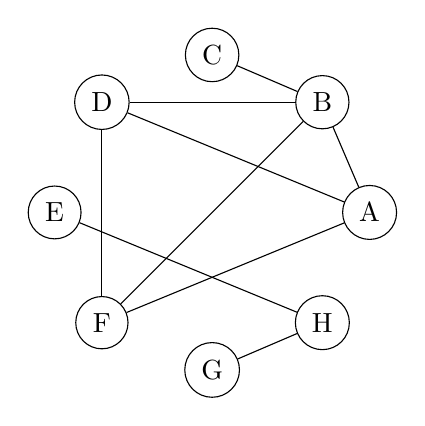
\begin{tikzpicture}
\node[shape=circle, draw=black](A) at (2,0) {A};
\node[shape=circle, draw=black](B) at (1.4,1.4) {B};
\node[shape=circle, draw=black](C) at (0,2) {C};
\node[shape=circle, draw=black](D) at (-1.4,1.4) {D};
\node[shape=circle, draw=black](E) at (-2,0) {E};
\node[shape=circle, draw=black](F) at (-1.4,-1.4) {F};
\node[shape=circle, draw=black](G) at (0,-2) {G};
\node[shape=circle, draw=black](H) at (1.4,-1.4) {H};

\draw (A) -- (B);
\draw (A) -- (D);
\draw (A) -- (F);
\draw (B) -- (D);
\draw (B) -- (F);
\draw (D) -- (F);
\draw (E) -- (H);
\draw (B) -- (C);
\draw (G) -- (H);
\end{tikzpicture}
\end{center}
The vertices $A,B,D,F$ form a clique of size $4$ on $G,$ and we also call this a \textit{fully connected subgraph} of $G.$ Similarly, the vertices $C,E,G$ form an anticlique on $G.$
\begin{defn}
A \textit{coloring} of some graph $G = (V,E)$ for some number of colors $c \in \NN$ is a partition of $E$ into $c$ partitions such that each edge is in only one partition.
\end{defn}
In general, a $k$-coloring of a particular set can refer (roughly) to a $k$-partitioning of that same set, with some constraints depending on context.

There are various different versions of Ramsey's Theorem, the first of which we will prove here.
\begin{thm}[Infinite Ramsey's Theorem]
\label{thm:IRT} If $G = (V,E)$ is an infinite graph, than $G$ either contains an infinite clique or infinite anticlique.
\end{thm}
\begin{proof}
Let $\xi \in \stt V \backslash V.$ By transfer, there exists $\xi, \stt \xi \in \stt \stt V$ for which there are two possibilities: either $(\xi, \stt \xi) \in \stt \stt E,$ or $(\xi, \stt \xi) \not\in \stt \stt E.$

We take the first case. We will recursively define a sequence $(v_1, \ldots, v_n)$ in $V$ such that $\{v_n \, | \, n \in \NN\}$ forms a clique in $G.$ Assume that there exists some $d \in \NN$ such that $v_0, \ldots , v_{d-1}$ are distinct vertices such that for $1 \leq i < j < d:$
\begin{itemize}
    \item $(v_i, v_j) \in E,$
    \item $(v_i, \xi) \in \stt E.$
\end{itemize}
There exists $x \in \stt V$ such that for all $i, x \neq v_i,$ and $(v_i, x) \in \stt E,$ and $(x, \stt \xi) \in \stt \stt E$ which is satisfied by $\xi.$ Then, therefore by transfer, there exists $x_d \in V$ different from $x_i$ for all $i$ such that $(x_i, x_d) \in E$ and $(x_d, \xi) \in \stt E.$ This process can be repeated ad infinitum, so there exists an infinite clique in $G.$

For the second case, the process is identical. Simply assume 
\begin{itemize}
    \item $(v_i, v_j) \not \in E,$
    \item $(v_i, \xi) \not \in \stt E.$
\end{itemize}
\end{proof}
This statement can be extended, however to do so we need the notion of a hypergraph. 
\begin{defn}
For some $n \in \NN,$ an $n$-regular hypergraph is a set of vertices $V$ together with a edge subset of $V^n$  $(\underset{n \text{ times}}{\underbrace{V \times V \times \cdots \times V}})$ called $E$ that is permutation-invariant and has the property that $(x_1, \ldots , x_n) \in E$ implies that $x_1, \ldots , x_n$ are pairwise distinct. A clique on the hypergraph $H = (V,E)$ is a subset $Y$ of $V$ such that for all $y_1, \ldots, y_n \in Y$ we have $(y_1, \ldots, y_n)\in E.$ An anticlique is defined similarly.
\end{defn}
Essentially, an $n$-regular hypergraph is a graph where the edges connect $n$ vertices such that all edges which contain the same vertices are equal and no vertex can have an edge to itself. For instance, the following is a $3$-regular hypergraph.
\begin{center}
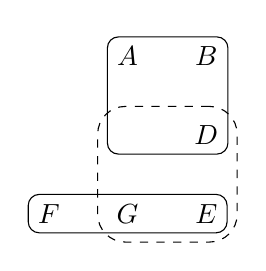
\begin{tikzpicture}
[
    he/.style={draw, rounded corners,inner sep=0pt},        % he = hyper edge
    ce/.style={draw,dashed, rounded corners=10pt}, % ce = condition edge
]

\node (f) at (0,0) {$F$};
\node (g) at (1,0) {$G$};
\node (e) at (2,0) {$E$};
\node (d) at (2,1) {$D$};
\node (a) at (1,2) {$A$};
\node (b) at (2,2) {$B$};

\node [he, fit=(f) (g) (e)] {};
\node [ce, fit=(g) (e) (d)] {};
\node [he, fit=(a) (d) (b)] {};
\node [fit=(a) (b) (d)] (fd){};
\end{tikzpicture}
\end{center}
Vertices $A,B,D$ are connected by an edge, $F,G,E$ are connected by an edge, and $D,G,E$ are connected by an edge. 
\begin{thm}[Infinite Ramsey's Theorem (Hypergraphs)]
\label{thm:irth} If $H = (V,E)$ is an infinite $n$-regular hypergraph, then $H$ contains either an infinite clique or an infinite anticlique.
\end{thm}
\begin{proof}
The method of proof is nearly identical to that of a standard graph. Let $\xi \in \stt V \backslash V.$ We consider the case where $n = 3.$ There are two cases, then: $(\xi, \stt \xi, \stt \stt \xi) \in \stt \stt \stt E$ or not.

We again will recursively define a sequence $(v_1, \ldots , v_m)$ such that it defines a clique in this hypergraph. Assume there exists $d \in \NN$ such that for $v_0, \ldots , v_{d-1}$ distinct elements of $V$ and all $1 \leq i < j < k < d$ we have:
\begin{itemize}
    \item $(v_i, v_j, v_k) \in E,$
    \item $(v_i, v_j, \xi) \in \stt E,$
    \item $(v_i, \xi, \stt \xi) \in \stt \stt E.$
\end{itemize}
Similarly, as before, there exists $x \in \stt V$ such that $x \neq v_0, \ldots , v_{d-1}$ and it satisfies $(x, \stt \xi, \stt \stt \xi) \in \stt \stt \stt E.$ Then, by transfer, there exists $x_d$ such that the above conditions are met, and this process can be repeated ad infinitum to generate a clique. 
For any arbitrary case $n,$ the process only differs in the amount of hyperextensions and the number of elements in the tuples you consider. For an anticlique, one simply takes the negations of the criteria.
\end{proof}
Now to state the infinite Ramsey's theorem in terms of colorings. For some set $X$ and $m \in \NN,$ we let $X^{[m]}$ be the set of $m$-element subsets of $X.$ This is often stated as 
\[X^{[m]}= \{(x_1, \ldots , x_m) \in X^m \, | \, x_1 < \cdots < x_m \},\] so that there is only one tuple associated with each subset. For some $k \in \NN,$ a $k$-coloring of $X^[m]$ is a function which maps each element in $X^{[m]}$ to a member of the set of naturals $\{1, \ldots , k\},$ and we refer to those mappings as colors. A subset $Y \subseteq X$ is monochromatic for some color if it only maps to a single color. 
\begin{cor}[Infinite Ramsey's Theorem (Colorings)]
\label{thm:irtc} For any arbitrary $k, m \in \NN,$ any infinite set $V,$ and any $k$-coloring $C$ of $V^{[m]},$ there is an infinite subset of $V$ that is monochromatic.
\end{cor}
\begin{proof}
Consider the case $k=2.$ We identify the coloring $C: V^{[m]} \rightarrow {1,2}$ with the $m$-regular hypergraph $H = (V,E)$ satisfying $(v_1, \ldots , v_m) \in E$ if and only if $C(\{v_1, \ldots , v_m \}=1$ for distinct $v_1, \ldots, v_m \in V.$ An infinite clique in $H$ corresponds to an infinite set with color 1, and an infinite anticlique in $H$ corresponds to an infinite set with color 2. By \ref{thm:irth}, there exists an infinite monochromatic subset of $V.$ For cases $k \geq 3,$ we can iteratively consider colorings in the same manner with the proof structure nearly identical.
\end{proof}
\section{Hindman's Theorem}
\begin{defn}
For some $B \subset \NN,$ the set of finite sums of distinct elements of $A$ is given by 
\[FS(B) =\left \{ b_D = \sum_{i \in D}b_i \, | \, D \subset B, D \text{ is finite}\right \}. \]
\end{defn}
\begin{thm}[Hindman's Theorem]
\label{thm:hindman} For every finite coloring of $\NN,$ there exists an infinite set $B \in \NN$ such that $FS(B)$ is monochromatic.
\end{thm}
The original combinatorical proof for this theorem is quite difficult, but using nonstandard methods eases the path slightly. However, we must define some additional machinery before we tackle it. 
\subsection{Ultrafilter Algebra} Let $\mcU, \mathcal{V}$ be ultrafilters on $\NN.$ 
\begin{defn}
We define the pseudo-sum operation $\oplus$ between two ultrafilters $\mcU, \mathcal{V}$ to be such that for some set $A \subseteq \NN,$
\[A \in \mcU \oplus \mathcal{V} \iff \{n | A - n \in \mathcal{V} \} \in \mcU, \]
where $A - n = \{ m \, | \, m+n \in A\}.$ This means that the pseudo-sum of two ultrafilters $\mcU$ and $\mathcal{V}$ is another ultrafilter over $\NN.$
\end{defn}
We can define multiplication similarly.
\begin{rem}
Generally, $\mcU_\xi \oplus \mcU_\zeta \neq \mcU_{\xi + \zeta}.$
\end{rem}
Following from this, we have that $\mcU_\xi \oplus \mcU_\zeta = \mcU_{\xi + \stt \zeta},$ and $\mcU_\xi \oplus \mcU_\zeta \oplus \mcU_{\mu} = \mcU_{\xi + \stt \zeta + \stt \stt \mu},$ and so on and so forth. 
\begin{defn}
An idempotent ultrafilter $\mcU$ is one such that \[\mcU \oplus \mcU = \mcU. \]
\end{defn}
Idempotent ultrafilters have some cool properties, namely that
\begin{itemize}
    \item $\mcU_\xi = \mcU_\xi \oplus \mcU_\xi,$
    \item $\xi + \stt \xi \underset{u}{\sim} \xi,$ and
    \item $\xi \in \stt A \Longrightarrow a + \xi \in \stt A$ for some $a \in A$
are all equivalent. We also define idempotent hypernaturals to be hypernaturals which generate idempotent ultrafilters. 
\end{itemize}
From this, we can define a proof of Hindman's theorem. 
\subsection{Proof} 
\begin{proof}
Let $\xi \in \stt \NN$ be an idempotent hypernatural, and let $C$ be the color of $\NN$ such that $\xi \in \stt C.$ We can then pick some $b_1 \in C$ such that $b_1 + \xi \in \stt C.$

Much similarly to our previous nonstandard proofs, we will use a recursive construction. Assume that there exists some sequence $b_1, \ldots, b_n$ for some $n \in \NN$ such that 
\begin{itemize}
    \item $b_D = \sum_{i \in D}b_i \in C,$
    \item $b_D + \xi \in \stt C$
\end{itemize}
for every $D \subseteq \{1, \ldots , n\}.$

We have that $\stt b_D + \stt \xi \in \stt \stt C$ by transfer, and by the properties of idempotents, $\stt \xi \in \stt \stt C$ implies that $\xi + \stt \xi \in \stt \stt C.$ And as $b_D$ is a finite natural number, this can be rewritten as $b_D + \xi + \stt \xi \in \stt \stt C.$

Combining this fact with $b_D + \xi \in \stt C,$ by transfer we find that $b_{n+1} > b_n$ exists such that $b_D + b_{n+1} \in C$ and $b_D + b_{n+1} + \xi \in \stt C$ for every $D.$
\end{proof}

\section{Partition Regularity of Diophantine Equations}
Let $F(X_1, \ldots, X_n)$ be a polynomial over $\ZZ.$
\begin{prop}
For some ultrafilter $\mcU$ over $\NN,$ the following two statements are equivalent: \label{sigmauf}
\begin{enumerate}
    \item For every $A \in \mcU,$ there are distinct $x_1, \ldots, x_n \in A$ such that $F(x_1, \ldots x_n)=0.$
    \item There exists $k \in \NN$ and distinct $\alpha_1, \ldots, \alpha_n \in {}^k\stt \NN$ such that $\mcU = \mcU_{\alpha_i}$ for all $i = 1, \ldots, n$ and $F(\alpha_1, \ldots, \alpha_n)=0.$
\end{enumerate}
Here we let $^k \stt \NN$ denote the $k$-th hyperextension of the natural numbers, i.e. ${}^{\underset{k \text{ times}}{\underbrace{**\cdots *}}}\NN.$
\end{prop}
\begin{proof}
Assume that the first statement holds. Then, for $A \in \mcU,$ set
\[X_A = \left \{ (\alpha_1, \ldots , \alpha_n ) \in \stt \NN ^n \, | \, \alpha_1, \ldots , \alpha_n \text{ are distinct}, \alpha_i \in \stt A, \stt F(\alpha_1, \ldots , \alpha_n) =0\right \}. \]
This family of sets has the FIP (\ref{fip}) so there exists $(\alpha_1, \ldots, \alpha_n) \in \cap_A X_a.$ This tuple satisfies the second statement.

Assume that the second statement holds. We then have $\alpha_1, \ldots , \alpha_n \in {}^k \stt \NN.$ Suppose that $A \in \mcU.$ There exist $i \in \{1,2 , \ldots r\}$ and distinct $x_1, \ldots, x_n \in \stt {}^k \stt A$ such that $F(x_1, \ldots , x_n)=0,$ and this statement is satisfied by $\alpha_1, \ldots , \alpha_n.$ This can be shown by repeated applying transfer $k$ times. 

\end{proof}
\begin{defn}
We call an ultrafilter satisfying \ref{sigmauf} an $[\iota_F]\sigma_F$-ultrafilter on $\NN.$
\end{defn}
\begin{defn}
$F(X_1, \ldots , X_n)=0$ is \textit{partition regular} $(PR)$ on $\NN$ if for every finite coloring of $\NN$ there exists a monochromatic solution. In other workds, for every finite partition $N = C_1 \cup \cdots \cup C_r,$ there exists some $i \in \{ 1, \ldots , r\}$ and distinct $x_1, \ldots , x_n \in C_i$ such that $F(x_1, \ldots , x_n) = 0.$
\end{defn}
\begin{prop} \label{ufimp}
$F(X_1, \ldots, X_n)$ is partition regular if and only if there exists a $[\iota_F]\sigma_F$-ultrafilter on $\NN.$
\end{prop}
\begin{proof}
We take the forward direction. Suppose that $F(X_1, \ldots, X_n)=0$ is partition regular. For some $A \subseteq \NN,$ consider the set 
\begin{multline*}
Y_A = \{(\alpha_1, \ldots , \alpha_n) \in \stt \NN ^n \, | \, \alpha_1, \ldots , \alpha_n \text{ are distinct}, \\ \bigwedge_{i,j}(\alpha_i \in \stt A \iff \alpha_j \in \stt A), \stt F(\alpha_1, \ldots , \alpha_n) = 0, 1 \leq i < j \leq n \}. 
\end{multline*}
Observe that the family $(Y_A)_{A \subseteq \NN}$ has the finite intersection property (FIP). For some $A_1, \ldots, A_m \subseteq \NN,$ let $A_i$ represent an arbitrary such set, $1 \leq i \leq m.$  Since $F(X_1, \ldots, X_n) = 0$ is partition regular, there is $j \in \{1, \ldots , k \}$ and distinct $x_1, \ldots , x_n \in A_i$ such that $F(x_1, \ldots , x_n) = 0.$ It then follows that $(x_1, \ldots , x_n) \in \bigcap ^{m}_{i=1} X_{A_i}.$ Then, it follows that there is $(\alpha_1, \ldots , \alpha_n) \in \bigcap_{A \subseteq \NN}Y_A.$ These $\alpha_1, \ldots , \alpha_n$ satisfy the conditions to make a $[\iota_F]\sigma_F$-ultrafilter.

For the opposite direction, the existence of $\alpha_1, \ldots, \alpha_n \in {}^k\stt \NN$ in the filter implies the partition regularity of $F(X_1, \ldots , X_n).$

\end{proof}
Some partition regular equations are 
\begin{align*}
    X + Y &= Z, \\
    X + Y &= 2Z. 
\end{align*}
To show this, we rely on two well known theorems:
\begin{thm}[Schur's Theorem] \label{schur}
In every finite coloring of $\NN$ one finds monochromatic triples $a,b,a+b.$
\end{thm}
As a result, $X + Y = Z$ is PR as the triple $a,b,a+b$ satisfies $X+Y-Z = 0$ for all colorings on $\NN.$
\begin{thm}[van der Waerden's Theorem] \label{Waerden}
In every finite coloring of $\NN$ one finds arbitrarily long arithmetic progressions.
\end{thm}
From this, we show that $X+Y=2Z$ is PR, by taking the existence of $3$-term arithmetic progressions $a, a+d, a+2d$ in every coloring of $\NN.$ Then, we have $X + Y - 2Z = 0$ satisfied by $a + a+d -2(a+d) = 0.$ However, we can also prove this with nonstandard methods.
\begin{cor}
$F(X_1, \ldots , X_n) = 0$ is partition regular on $\NN$ if there exist $\xi_1 \underset{u}{\sim} \cdots \underset{u}{\sim} \xi_n$ in $\stt \NN$ such that $\stt F(\xi_1, \ldots, \xi_n) =0.$
\end{cor}
This follows from \ref{ufimp}.
\begin{thm}[Bergelson-Hindman 1990]
Let $\mcU$ be an idempotent ultrafilter on $\NN.$ Then every $A \in 2\mcU \oplus \mcU$ contains an arithmetic progression of length 3. In consequence, $X-2Y+Z=0$ is partition regular. 
\end{thm}
\begin{proof}
Let $v$ satisfy $\mcU = \mcU_v.$ It follows that $v \underset{u}{\sim} v + \stt v,$ by the properties of idempotents. Then, we can define the infinitesimals
\begin{itemize}
    \item $\xi = 2v + \stt \stt v,$
    \item $\zeta = 2v + \stt v + \stt \stt v,$
    \item $\mu = 2v + 2 \stt v + \stt \stt v.$
\end{itemize}
Observe that $\xi \underset{u}{\sim} \zeta \underset{u}{\sim} \mu \in \stt \stt \stt \NN.$ Additionally, they generate the ultrafilter $\mathcal{V} = 2\mcU \oplus \mcU.$ For every $A \in \mathcal{V},$ we have that $\xi, \zeta, \mu \in \stt \stt \stt A$ form a $3$-term arithmetic progression, and therefore by transfer there exists a $3$-term arithmetic progression in $A.$ The terms in this arithmetic progression satisfy $X - 2Y + Z = 0,$ making the equation partition regular.
\end{proof}
\section{Rado's Theorem} 
Rado's Theorem defines the partition regularity of linear Diophantine equations, and can be stated as follows:
\begin{thm}[Rado's Theorem] \label{rado}
The Diophantine equation $c_1X_1 + \cdots + c_nX_n =0$ is partition regular if and only if $\sum_{i \in I}c_i = 0$ for some nonempty $I \subseteq \{1, \ldots , k\}.$
\end{thm}
Let \[P(x) = \sum_{j=0}^n b_j X^j \in \ZZ[X]\] and $\xi \in \stt \ZZ.$ Then, we define \[\tilde{P}(\xi) = \sum_{j=0}^n b_j {}^j \stt \xi \in {}^{j+1}\stt \ZZ.\]
\begin{lemma} \label{105}
Suppose that $c_1, \ldots , c_k \in \ZZ$ are such that there exist distinct polynomials $P_1(X), \ldots , P_k(X) \in \ZZ[X]$ and $\xi, \eta \in \stt \NN$ for which
\begin{enumerate}
    \item $c_1P_1(X) + \cdots + c_kP_k(X) = 0,$
    \item $\tilde{P}_i(\xi) \underset{u}{\sim} \eta$ for each $i = 1, \ldots , k.$
\end{enumerate}
Then, $\mcU_\eta$ witnesses that $c_1X_1 + \ldots + c_kX_k = 0$ is partition regular.
\end{lemma}
\begin{proof}
For each $i = 1, \ldots , k,$ let $\alpha_i = \tilde{P}(\xi).$ From our assumption, we have that $\mcU_{\alpha_i} = \mcU_\eta$ for all $i,$ and that $c_1 \alpha_1 + \cdots + c_k \alpha_k = 0.$ Then, we have that $\mcU_\eta$ witnesses that $c_1X_1 + \cdots + c_kX_k=0$ is partition regular. 

Additionally, assuming that the polynomials $P_i$ are distinct, to show partition regularity we must show that all $\alpha_i$ are distinct. We show this by contradiction. Suppose that $\alpha_i = \alpha_j.$ This implies that $\tilde{P}_i(\xi) = \tilde{P}_j(\xi).$ Then, we write
\begin{align*}
    P_i(X) &= \sum_{l=0}^m r_lX^l, \\
    P_j(X) &= \sum_{l=0}^m s_lX^l.
\end{align*}
With substitution and some algebraic manipulations, we get 
\[(r_m - s_m)^m\stt \xi = - \sum_{l=0}^{m-1} (r_l-s_l)^l \stt \xi. \] This is only satisfied when $r_m = s_m = 0,$ and proceeding with the same process we determine that $P_i = P_j,$ a contradiction.
\end{proof}
\begin{defn}
We define the equivalence relation $\approx_u$ on finite strings of integers to be the smallest equivalence relation satisfying the following three properties:
\begin{itemize}
    \item $\emptyset \approx_u \langle 0 \rangle.$
    \item If $a \in \ZZ,$ then $\langle a \rangle \approx_u \langle a, a \rangle,$
    \item If $\sigma \approx_u \sigma '$ and $\tau \approx_u \tau ',$ the concatenations $\sigma \tau \approx_u \sigma ' \tau '.$
\end{itemize}
If $P,Q \in \ZZ[X]$ are polynomials, then we write $P \approx_u Q$ to say that their strings of coefficients are $u$-equivalent.
\end{defn}
In essence, this version of $u$-equivalence is the smallest equivalence relation such that the empty sting maps to $0,$ strings containing the same term are equivalent, and it is coherent with concatenations. As an example, we have
\begin{align*}
    \langle 1,2,0,4,4,7,5,6,0 \rangle & \approx_u \langle 1,0,2,2,4,7,5,5,6\rangle \\
    &\approx_u \langle 1,2,4,7,5,6\rangle .
\end{align*}
So, $u$-equivalence is preserved by inserting or removing zeroes, repeating a term finitely many times, and shortening series of consecutive equal terms.
\begin{lemma} \label{107}
Let $P,Q \in \ZZ[X]$ have positive leading coefficients. If $P \approx_u Q,$ then for every idempotent $\xi \in \stt \NN,$ we have $\tilde{P}(\xi) \sim \tilde{Q}(\xi).$
\end{lemma}
\begin{proof}
Fix an idempotent $\xi \in \stt \NN.$ Then, the following is true:
\begin{align*}
    \sum_{j=0}^m a_j {}^j \stt \xi &\sim \sum_{j=0}^i a_j {}^j \stt \xi + a_i^{(i+1)}\stt \xi + \sum_{j=i+1}^m a_j^{(j+1)} \stt \xi.
\end{align*}
Additionally, if we have
\begin{align*}
    \sum_{j=0}^m a_j {}^j\stt \xi &\sim \sum_{j=0}^{m'}a'_j {}^j \stt \xi, \\
    \sum_{j=0}^m b_j {}^j\stt \xi &\sim \sum_{j=0}^{m'}b'_j {}^j \stt \xi,
\end{align*}
then it follows that 
\[ \sum_{j=0}^m a_j {}^j\stt \xi + \sum_{j=0}^n b_j {}^{(j+m)}\stt \xi \sim \sum_{j=0}^{m'} a'_j {}^j\stt \xi + \sum_{j=0}^{n'} b'_j {}^{(j+m')}\stt \xi.\]
From this, by the definition of $\tilde{P}(\xi),$ we see that $\tilde{P}(\xi) \sim \tilde{Q}(\xi).$
\end{proof}
Now, we can prove Rado's Theorem in a more specific form.
\begin{cor} \label{thecorrolary}
Suppose that $k>2$ and $c_1, \ldots , c_k \in \ZZ$ are such that $c_1 + \cdots c_k = 0.$ Then there exists $a_0, \ldots , a_{k-2} \in \NN$ such that, for every idempotent ultrafilter $\mcU,$ we have that $a_0 \mcU \oplus \cdots \oplus a_{k-2}\mcU$ witnesses the partition regularity of the equation $c_1X_1 + \ldots + c_kX_k = 0.$
\end{cor}
\begin{proof}
Without loss of generality, assume that $c_1 \geq c_2 \geq \cdots \geq c_k.$ By Lemmas \ref{105} and \ref{107}, we need to find $a_0, \ldots , a_{k-2} \in \NN$ and distinct $P_1(X), \ldots, P_k(X) \in N_0[X]$ such that $c_1P_1(X) + \cdots + c_kP_k(X) = 0$ and such that $P_i(X) \approx_u \sum_{j=0}^{k-2}a_jX^j$ for each $i = 1, \ldots , k.$ We define the following polynomials:
\begin{align*}
    P_1(X) &= \sum_{j=0}^{k-2} a_jX^j + a_{k-2}X^{k+1}, \\
    P_i(X) &= \sum_{j=0}^{k-i-1} a_jX^j + \sum_{j=k-i+1}^{k-1}a_{j-1}X^j, \\
    P_k(X) &= a_0 + \sum_{j=1}^{k-1} a_{j-1}X^j.
\end{align*}
The definition for $P_i$ holds for $2\leq i \leq k-1.$ 

We can check that $P_i(X) \approx_u \sum_{j=0}^{k-2} a_j X^j$ for each $i = 1, \ldots , k.$ Additionally, because $a_0, \ldots , a_{k-2}$ are nonzero, then the polynomials $P_1(X) ,\ldots , P_k(X)$ are mutually distinct. Then, therefore, we must show that there exist $a_0, \ldots, a_{k-2} \in \NN$ such that the conditions are satisfied. 

Since $c_1 + \cdots + c_k = 0,$ the constant and leading terms of $c_1P_1(X) + \cdots + c_kP_k(X)$ are zero. Then, the equation $c_1P_1(X) + \cdots + c_kP_k(X) = 0$ is equivalent to the system of equations $(c_1 + \cdots + c_{k-i}) \cdot a_{i-1} + (c_{k-i+2} + \cdots + c_k)\cdot a_{i-2}$ for $i = 1,2, \ldots, k-1.$ Then, one can recursively define the elements $a_0, a_1, \ldots , a_{k-2}$ satisfying these equations, which completes the proof.
\end{proof}
And, therefore, we can prove Rado's Theorem.
\begin{proof}
Rado's Theorem \ref{rado} is a trivial result of Corollary \ref{thecorrolary}.
\end{proof}
For a more thorough exposition of topics in Ramsey theory and combinatorical number theory with nonstandard methods, look in \cite{Di19}.
\section{Acknowledgements}
The author would like to thank Maxim Giulia for insightful conversations on the topic, and Euler Circle and Simon Rubinstein-Salzedo for making this paper possible.
\bibliographystyle{alpha}
\bibliography{biblio}
\end{document}